\chapter{Anhang}

\begin{figure}
	\centering
	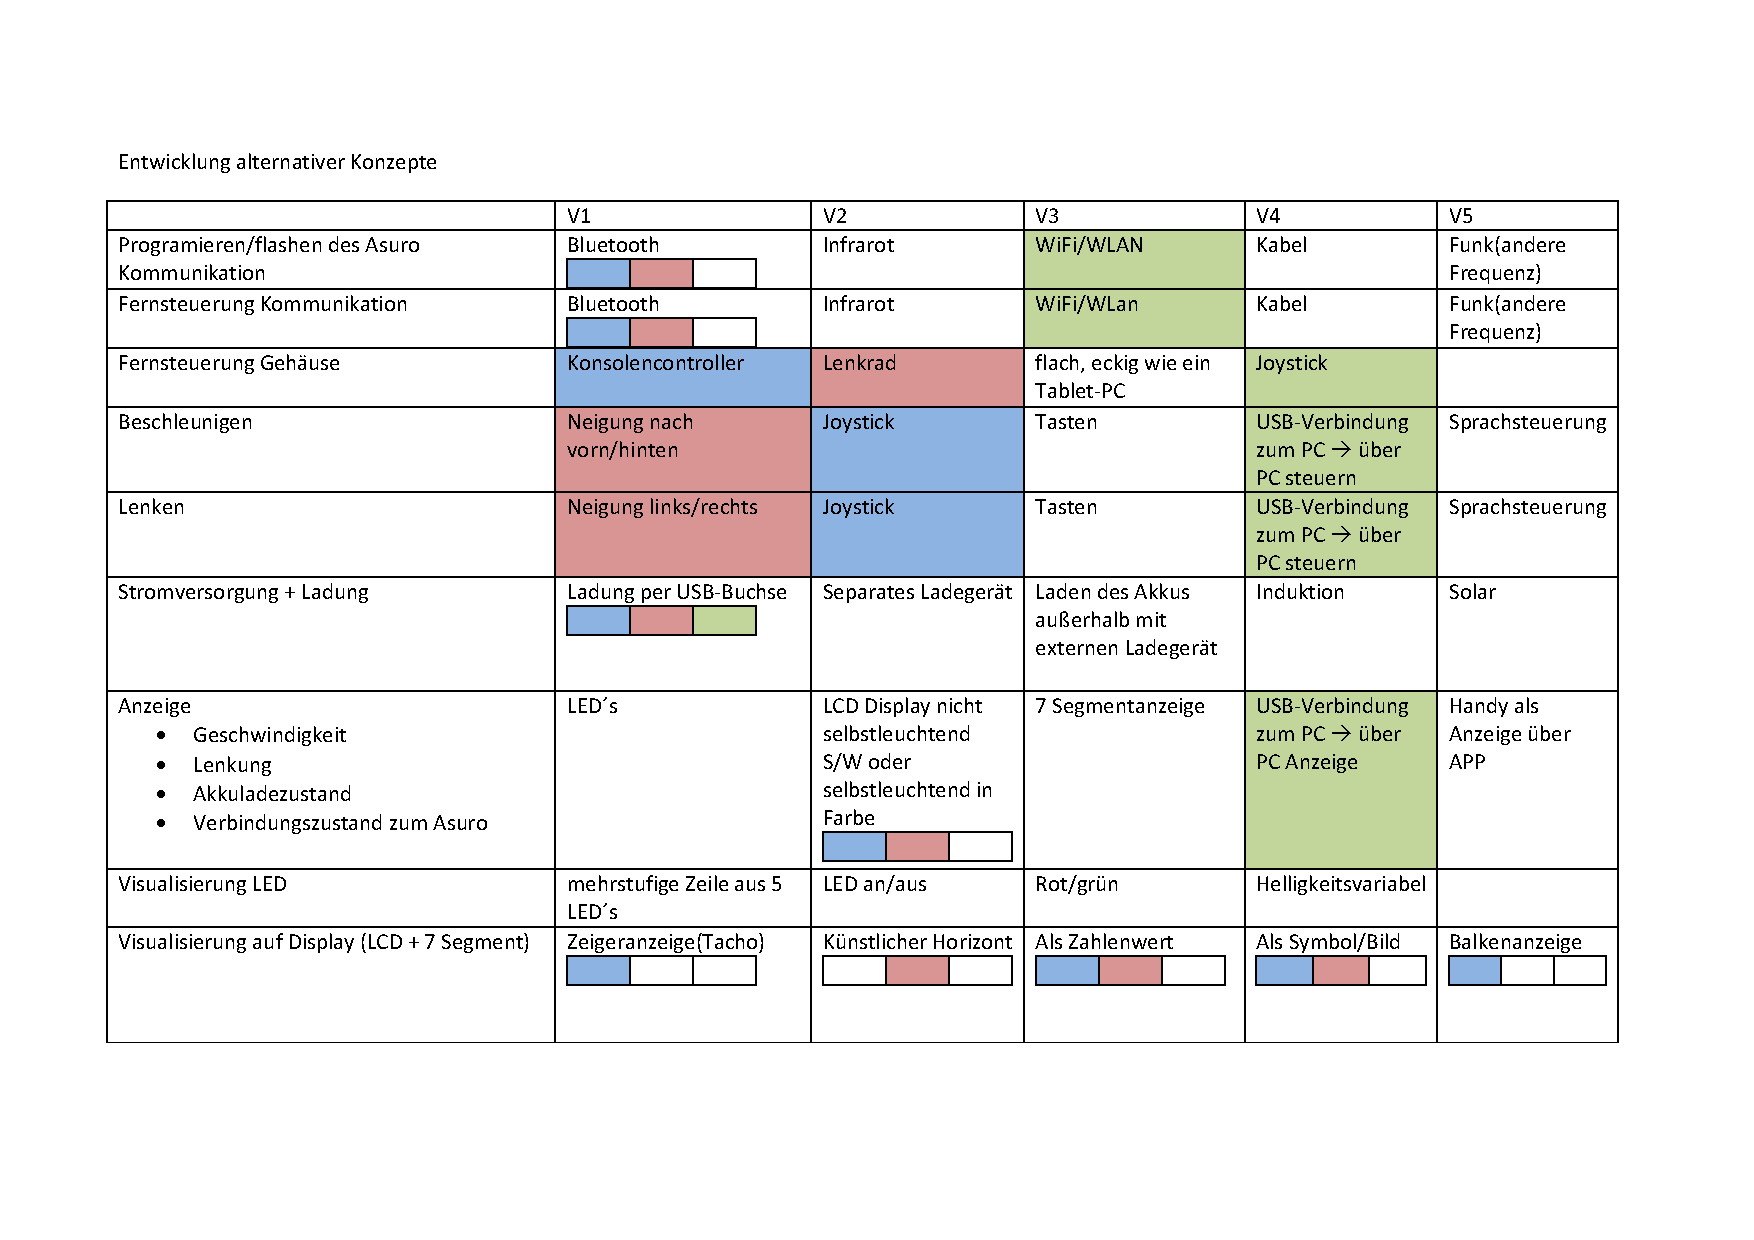
\includegraphics[angle=90, width=\textwidth]{konzepte_v1/Konzepte.pdf}
	\caption{Konzept-Übersicht}
	\label{fig:konzepte}
\end{figure}

% Konzepte, erste Version
\begin{figure}
	\centering
	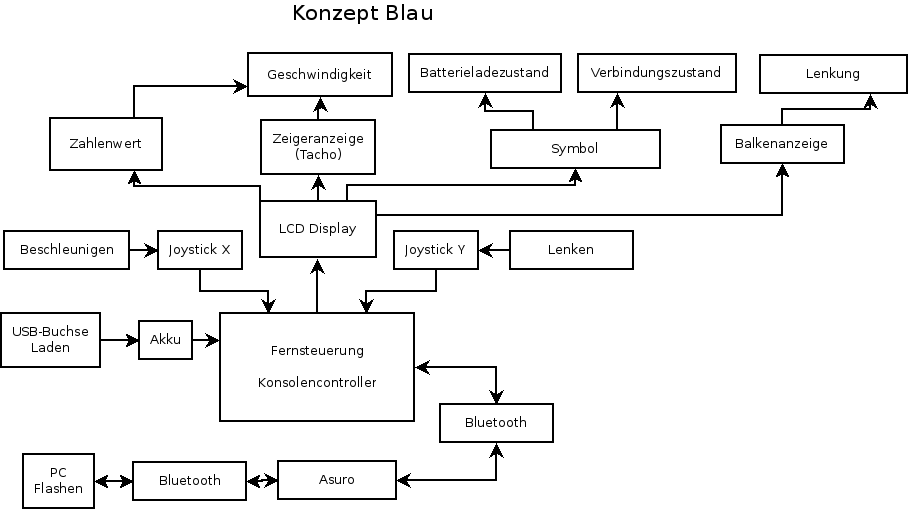
\includegraphics[width=\textwidth]{konzepte_v1/Konzept_Blau.png}
	\label{fig:blau_v1}
	\caption{Konzept Blau, Version 1}
\end{figure}

\begin{figure}
	\centering
	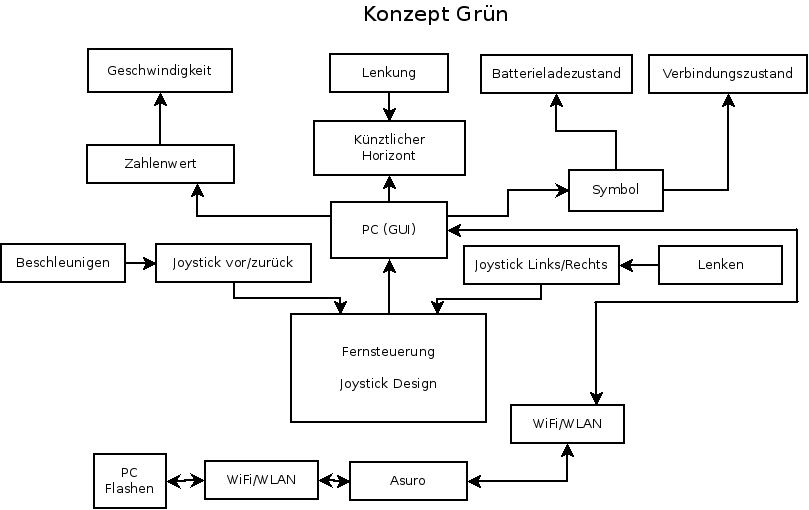
\includegraphics[width=\textwidth]{konzepte_v1/Konzept_Gruen.png}
	\caption{Konzept Grün, Version 1}
	\label{fig:gruen_v1}
\end{figure}

\begin{figure}
	\centering
	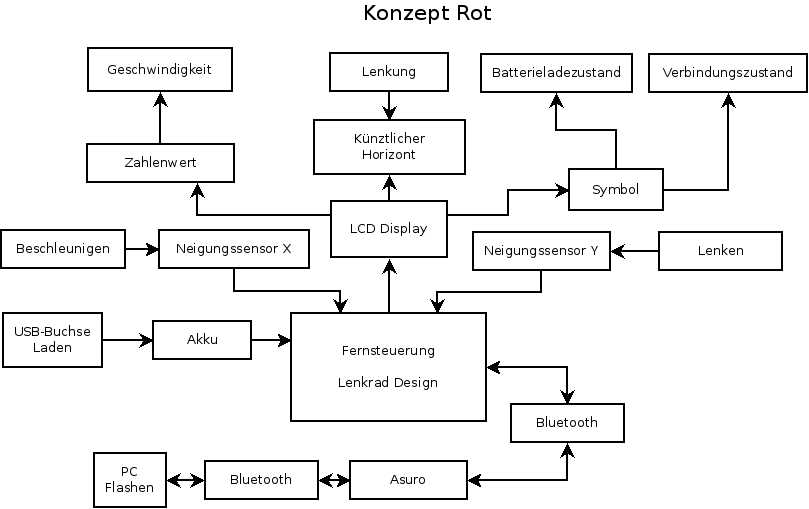
\includegraphics[width=\textwidth]{konzepte_v1/Konzept_Rot.png}
	\caption{Konzept Rot, Version 1}
	\label{fig:rot_v1}
\end{figure}

% Konzepte, zweite Version
\begin{figure}
	\centering
	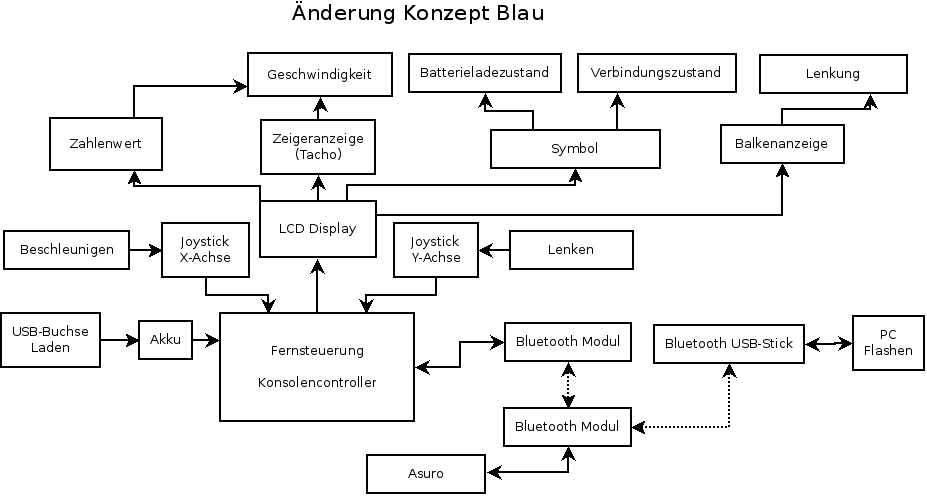
\includegraphics[width=\textwidth]{konzepte_v2/Konzept_Blau.png}
	\caption{Konzept Blau, Version 2}
	\label{fig:blau_v2}
\end{figure}

\begin{figure}
	\centering
	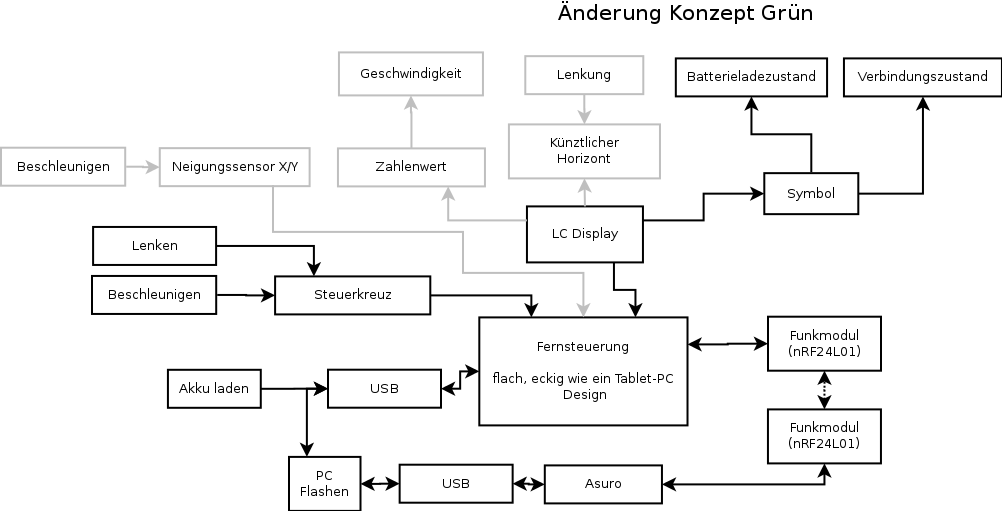
\includegraphics[width=\textwidth]{konzepte_v2/Konzept_Gruen.png}
	\caption{Konzept Grün, Version 2}
	\label{fig:gruen_v2}
\end{figure}

\begin{figure}
	\centering
	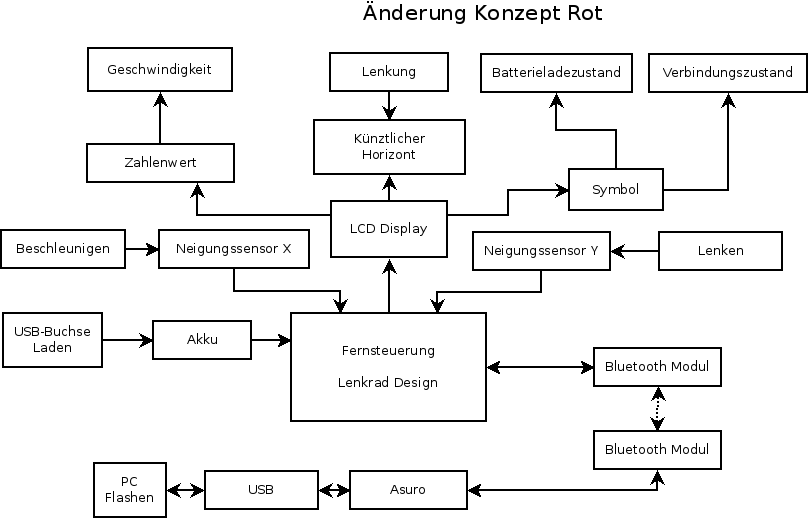
\includegraphics[width=\textwidth]{konzepte_v2/Konzept_Rot.png}
	\caption{Konzept Rot, Version 2}
	\label{fig:rot_v2}
\end{figure}
